
\section{Referencial teórico}

\begin{frame}{Lógica proposicional}{Sintaxe}
	\vspace{-.2cm}
	\begin{footnotesize}
	\begin{block}{Símbolos proposicionais}
		$\mathcal{P} = \{a,b,...,a_1,a_2,...,b_1,b_2,... \}$ é dito o conjunto de \emph{símbolos proposicionais}.
	\end{block}
	\pause
	\vspace{-.2cm}
	\begin{block}{Fórmulas}
		Se $\phi \in \mathcal{P}$, então $\phi$ é uma \emph{fórmula}. Além disso, se $\phi_1,...,\phi_n$, $n \in \mathbb{N} \cup \{0 \}$, são fórmulas, então também são:
		\begin{enumerate}
			\pause\item \emph{Negação}: $\neg \phi_1$
			\pause\item \emph{Conjunção}: $\phi_1 \wedge ... \wedge \phi_n$
			\pause\item \emph{Disjunção}: $\phi_1 \vee ... \vee \phi_n$
			\pause\item \emph{Implicação}: $\phi_1 \rightarrow \phi_2$
			\pause\item \emph{Equivalência}: $\phi_1 \leftrightarrow \phi_2$
		\end{enumerate}
		\pause Denotamos o conjunto de fórmulas por $\mathcal{L}$.
	\end{block}
	\end{footnotesize}
\end{frame}

\begin{frame}{Lógica proposicional}{Sintaxe -- Subfórmulas}
	\begin{block}{Subfórmulas imediatas}
		Na definição anterior, as fórmulas $\phi_i$ são \emph{subfórmulas imediatas}.
	\end{block}
	
	\pause
	\begin{block}{Subfórmulas próprias}
		Dizemos que $\psi$ é \emph{subfórmula própria de $\phi$} se $\psi$ é subfórmula imediata de $\phi$, ou se $\psi$ é subfórmula própria de $\xi$ e $\xi$ é subfórmula imediata de $\phi$.
		
		\pause Notação: $\psi \sqsubset \phi$ e $\{\psi \mid \psi \sqsubset \phi \} = SF(\phi)$
	\end{block}
\end{frame}

\begin{frame}{Lógica proposicional}{Semântica}
	\vspace{-.3cm}
	\begin{footnotesize}
	\begin{block}{Valorações booleanas}
		Dizemos que $\mathbb{v}_0$ é uma \emph{valoração booleana} se $\mathbb{v}_0 : \mathcal{P} \longmapsto \{V,F \}$.
	\end{block}
	\pause
	\vspace{-.2cm}
	\begin{block}{Interpretações}
		Seja $\mathbb{v}_0$ é uma valoração booleana. Dizemos que $\mathbb{v} : \mathcal{L} \longmapsto \{V,F \}$ é uma \emph{interpretação definida por $\mathbb{v}_0$}, se:
		\begin{enumerate}
			\pause\item Se $\phi_1 \in \mathcal{P}$, então $\mathbb{v}(\phi_1) = \mathbb{v}_0(\phi_1)$.
			\pause\item $\mathbb{v}(\neg \phi_1) = V$ se, e somente se, $\mathbb{v}(\phi_1) = F$.
			\pause\item $\mathbb{v}(\phi_1 \wedge ... \wedge \phi_n) = V$ se, e somente se, $\mathbb{v}(\phi_i) = V$, para todo $i$.
			\pause\item $\mathbb{v}(\phi_1 \vee ... \vee \phi_n) = V$ se, e somente se, $\mathbb{v}(\phi_i) = V$, para algum $i$.
			\pause\item $\mathbb{v}(\phi_1 \rightarrow \phi_2) = V$ se, e somente se, $\mathbb{v}(\phi_1) = F$ ou $\mathbb{v}(\phi_2) = V$.
			\pause\item $\mathbb{v}(\phi_1 \leftrightarrow \phi_2) = V$ se, e somente se, $\mathbb{v}(\phi_1) = \mathbb{v}(\phi_2)$.
		\end{enumerate}
	\end{block}
	\end{footnotesize}
\end{frame}

\begin{frame}{Lógica proposicional}{Semântica -- Algumas definições}
	\begin{enumerate}
		\item Se existe $\mathbb{v}$ tal que $\mathbb{v}(\phi) = V$, dizemos que $\phi$ é \emph{satisfatível}.
		\pause\item Se $\mathbb{v}(\phi) = F$ para toda $\mathbb{v}$, dizemos que $\phi$ é \emph{insatisfatível}.
		\pause\item Se $\mathbb{v}(\phi) = V$ para toda $\mathbb{v}$, dizemos que $\phi$ é uma \emph{tautologia}.
	\end{enumerate}
\end{frame}

\begin{frame}{Problemas da lógica proposicional}
	Seja $L \subseteq \mathcal{L}$. Se nos referimos a $L$ como um \emph{problema}, referimo-nos ao problema de, dada $\phi$ qualquer, determinar se $\phi \in L$ ou se $\phi \notin L$.
	\vspace{-.3cm}
	\begin{enumerate}
		\pause\item $\text{SAT} = \{\phi \in \mathcal{L} \mid \phi \text{ é satisfatível} \}$
		\pause\item $\text{UNSAT} = \{\phi \in \mathcal{L} \mid \phi \text{ é insatisfatível} \}\pause = \overline{\text{SAT}}$
		\pause\item $\text{VAL} = \{\phi \in \mathcal{L} \mid \phi \text{ é tautologia} \}$
	\end{enumerate}
	
	\vspace{.2cm}
	\pause $$\phi \in \text{VAL} \iff \neg \phi \in \text{UNSAT} \iff \neg \phi \notin \text{SAT}$$
\end{frame}

\begin{frame}{Formas normais}{Regras de reescrita}
	Uma \emph{regra de reescrita} que transforma $\phi$ em $\psi$, escrito $\phi \longmapsto \psi$,
	\begin{enumerate}
		\pause\item \emph{preserva equivalência} se, e somente se, $\mathbb{v}(\phi) = \mathbb{v}(\psi), \forall \mathbb{v}$.
		\pause\item \emph{preserva satisfatibilidade} se, e somente se, $\phi,\psi \in \text{SAT}$ ou $\phi,\psi \notin \text{SAT}$.
	\end{enumerate}
\end{frame}

\begin{frame}{Formas normais}{Forma normal negada (FNN)}
	$$(p \wedge \neg q \wedge \neg r) \vee (x \wedge \neg y \wedge (r \vee s))$$
	
	\pause As transformações:
	\begin{enumerate}
		\item $\neg \neg \phi_1 \longmapsto \phi_1$ \;\; (eliminação de dupla negação)
		\item $\neg(\phi_1 \wedge ... \wedge \phi_n) \longmapsto \neg \phi_1 \vee ... \vee \neg \phi_n$ \;\; (De Morgan)
		\item $\neg(\phi_1 \vee ... \vee \phi_n) \longmapsto \neg \phi_1 \wedge ... \wedge \neg \phi_n$ \;\; (De Morgan)
		\item $\phi_1 \rightarrow \phi_2 \longmapsto \neg \phi_1 \vee \phi_2$
		\item $\phi_1 \leftrightarrow \phi_2 \longmapsto (\phi_1 \rightarrow \phi_2) \wedge (\phi_2 \rightarrow \phi_1)$
	\end{enumerate}
	\pause preservam equivalência!
\end{frame}

\begin{frame}{Formas normais}{Forma normal clausal (FNC)}
	$$(p \vee \neg q \vee \neg r) \wedge (x \vee \neg y \vee r \vee s) \wedge (a \vee \neg b \vee c)$$
	
	\pause A transformação:
	\begin{center}
		$\phi \vee (\psi \wedge \xi) \longmapsto (\phi \vee \psi) \wedge (\phi \vee \xi)$ \;\; (distribuição)
	\end{center}
	\pause preserva equivalência!
	
	\vspace{.5cm}
	\pause Geralmente provoca crescimento exponencial!
\end{frame}

\begin{frame}{Renomeamento}
	\begin{enumerate}
		\item Escolhemos um conjunto de subfórmulas $R \subseteq SF(\phi)$.
		\pause\item Para cada $\psi \in R$:
		\begin{enumerate}
			\pause\item Escolhemos um símbolo proposicional novo $s(\psi) \in \mathcal{P}$.
			\pause\item Trocamos todas as ocorrências de $\psi$ por $s(\psi)$.
			\pause\item Incluímos a definição $s(\psi) \rightarrow \psi$ em conjunção.
		\end{enumerate}
	\end{enumerate}
	
	\begin{small}
	\pause Exemplo: $(\neg p_1 \wedge p_2 \wedge p_3) \vee (\neg q_1 \wedge q_2 \wedge \neg q_3)$\\
	\pause Seja $\phi_1 = \neg p_1 \wedge p_2 \wedge p_3$.\\
	\pause Escolhendo $R = \{\phi_1 \}$ e $s(\phi_1) = a$, temos\pause $$(a \vee (\neg q_1 \wedge q_2 \wedge \neg q_3)) \wedge (a \rightarrow (\neg p_1 \wedge p_2 \wedge p_3))$$
	
	\pause Não preserva equivalência. \pause Mas preserva satisfatibilidade!
	\end{small}
\end{frame}

\begin{frame}{Reduzindo o número de cláusulas}{Contando cláusulas}
	Denotamos o \emph{número de cláusulas} geradas por $\phi$ ao ser colocada na FNC por $p(\phi)$.
	\pause
	\begin{center}
	\begin{tabular}{c|c}
		Forma de $\phi$                   & $p(\phi)$                                 \\ \hline
		$\phi_1 \wedge ... \wedge \phi_n$ & $p(\phi_1) + ... + p(\phi_n)$                                  \\
		$\phi_1 \vee ... \vee \phi_n$     & $p(\phi_1) \cdot ... \cdot p(\phi_n)$                       \\
		$x \text{ ou } \neg x, x \in \mathcal{P}$            & $1$                                                             \\
	\end{tabular}
	\end{center}
	
	\pause Exemplo: $\phi = (\neg p_1 \wedge p_2 \wedge p_3) \vee (\neg q_1 \wedge q_2 \wedge \neg q_3) \vee (r_1 \wedge r_2 \wedge \neg r_3)$\\
	\pause Temos que $$p(\phi) = (1 + 1 + 1)(1 + 1 + 1)(1 + 1 + 1) = 3^3 = 27$$
\end{frame}

\begin{frame}{Reduzindo o número de cláusulas}{O problema}
	\begin{block}{Problema}
		Escolher $R \subseteq SF(\phi)$ de modo que o número de cláusulas $p(\phi,R)$ da transformação por renomeamento seja mínimo.
	\end{block}
\end{frame}

\begin{frame}{Reduzindo o número de cláusulas}{Algoritmo de Boy de la Tour}
	\begin{block}{Árvores lineares}
		Seja $\phi$ uma fórmula na FNN. Se cada subfórmula de $\phi$ ocorre somente uma vez, dizemos que $\phi$ é uma \emph{árvore linear}.
	\end{block}
	
	\pause Se $\phi$ é uma árvore linear, o algoritmo de Boy de la Tour encontra um conjunto $R \subseteq SF(\phi)$ tal que $p(\phi,R)$ é ótimo (mínimo).
	
	\vspace{.1cm}
	\pause Seu custo de tempo no pior caso é $O(|SF(\phi)|^2)$.
\end{frame}

\begin{frame}{Reduzindo o número de cláusulas}{Algoritmo de Boy de la Tour}
	O algoritmo escreve o número de cláusulas na forma irredutível $$p(\phi) = c + a_\psi^\phi \cdot p(\psi)$$
	
	\pause Logo, se $R = \{\psi \}$, então $$p(\phi,R) = c + a_\psi^\phi + p(\psi)$$
	
	\pause Assim, é feita em $\phi$ uma busca em profundidade pré-ordem, incluindo em $R$ cada $\psi \sqsubset \phi$ que satisfaz $$a_\psi^\phi \cdot p(\psi) > a_\psi^\phi + p(\psi)$$
\end{frame}

\begin{frame}{Reduzindo o número de cláusulas}{Algoritmo de Boy de la Tour -- Exemplo}
	$$\phi = (\neg p_1 \wedge p_2 \wedge p_3) \vee (\neg q_1 \wedge q_2 \wedge \neg q_3) \vee (r_1 \wedge r_2 \wedge \neg r_3)$$
	
	\pause
	\begin{figure}
		\centering
		
		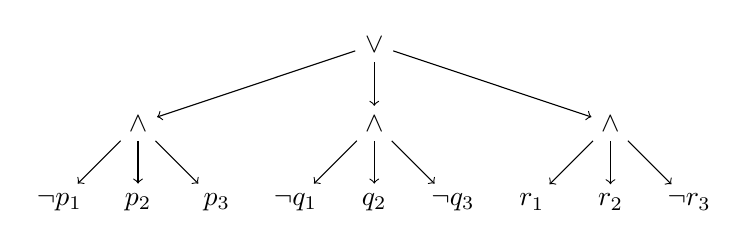
\begin{tikzpicture}
		\tikzset{vertex/.style = {}}
		\tikzset{edge/.style = {->}}
		
		\node[vertex]  (1) at (   0,    1) {$\vee$};
		\node[vertex]  (2) at (  -3,    0) {$\wedge$};
		\node[vertex]  (3) at (   0,    0) {$\wedge$};
		\node[vertex]  (4) at (   3,    0) {$\wedge$};
		\node[vertex]  (5) at (  -4,   -1) {$\neg p_1$};
		\node[vertex]  (6) at (  -3,   -1) {$p_2$};
		\node[vertex]  (7) at (  -2,   -1) {$p_3$};
		\node[vertex]  (8) at (  -1,   -1) {$\neg q_1$};
		\node[vertex]  (9) at (   0,   -1) {$q_2$};
		\node[vertex] (10) at (   1,   -1) {$\neg q_3$};
		\node[vertex] (11) at (   2,   -1) {$r_1$};
		\node[vertex] (12) at (   3,   -1) {$r_2$};
		\node[vertex] (13) at (   4,   -1) {$\neg r_3$};
		
		\draw[edge] (1) to  (2);
		\draw[edge] (1) to  (3);
		\draw[edge] (1) to  (4);
		\draw[edge] (2) to  (5);
		\draw[edge] (2) to  (6);
		\draw[edge] (2) to  (7);
		\draw[edge] (3) to  (8);
		\draw[edge] (3) to  (9);
		\draw[edge] (3) to (10);
		\draw[edge] (4) to (11);
		\draw[edge] (4) to (12);
		\draw[edge] (4) to (13);
		\end{tikzpicture}
	\end{figure}
\end{frame}

\begin{frame}{Reduzindo o número de cláusulas}{Algoritmo de Boy de la Tour -- Exemplo}
	\begin{figure}
		\centering
		
		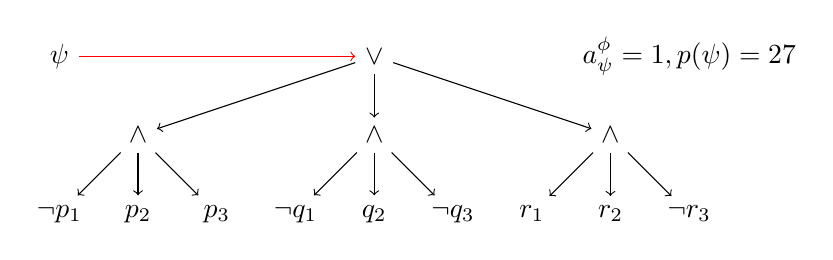
\begin{tikzpicture}
		\tikzset{vertex/.style = {}}
		\tikzset{edge/.style = {->}}
		
		\node[vertex]  (1) at (   0,    1) {$\vee$};
		\node[vertex]  (2) at (  -3,    0) {$\wedge$};
		\node[vertex]  (3) at (   0,    0) {$\wedge$};
		\node[vertex]  (4) at (   3,    0) {$\wedge$};
		\node[vertex]  (5) at (  -4,   -1) {$\neg p_1$};
		\node[vertex]  (6) at (  -3,   -1) {$p_2$};
		\node[vertex]  (7) at (  -2,   -1) {$p_3$};
		\node[vertex]  (8) at (  -1,   -1) {$\neg q_1$};
		\node[vertex]  (9) at (   0,   -1) {$q_2$};
		\node[vertex] (10) at (   1,   -1) {$\neg q_3$};
		\node[vertex] (11) at (   2,   -1) {$r_1$};
		\node[vertex] (12) at (   3,   -1) {$r_2$};
		\node[vertex] (13) at (   4,   -1) {$\neg r_3$};
		
		\node[vertex] (14) at (  -4,    1) {$\psi$};
		
		\node[vertex] (15) at (   4,    1) {$a_\psi^\phi = 1, p(\psi) = 27$};
		
		\draw[edge] (1) to  (2);
		\draw[edge] (1) to  (3);
		\draw[edge] (1) to  (4);
		\draw[edge] (2) to  (5);
		\draw[edge] (2) to  (6);
		\draw[edge] (2) to  (7);
		\draw[edge] (3) to  (8);
		\draw[edge] (3) to  (9);
		\draw[edge] (3) to (10);
		\draw[edge] (4) to (11);
		\draw[edge] (4) to (12);
		\draw[edge] (4) to (13);
		
		\tikzset{edge/.style = {->,red}}
		\draw[edge] (14) to (1);
		\end{tikzpicture}
	\end{figure}
\end{frame}

\begin{frame}{Reduzindo o número de cláusulas}{Algoritmo de Boy de la Tour -- Exemplo}
	\begin{figure}
		\centering
		
		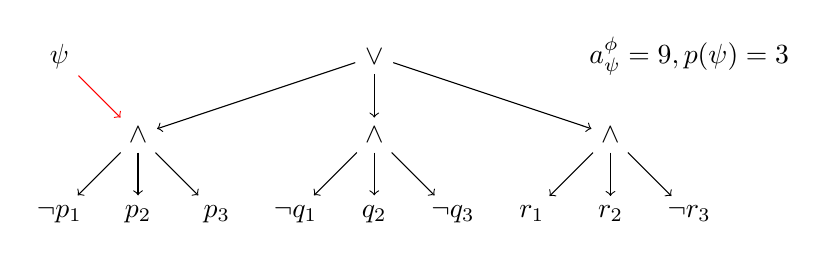
\begin{tikzpicture}
		\tikzset{vertex/.style = {}}
		\tikzset{edge/.style = {->}}
		
		\node[vertex]  (1) at (   0,    1) {$\vee$};
		\node[vertex]  (2) at (  -3,    0) {$\wedge$};
		\node[vertex]  (3) at (   0,    0) {$\wedge$};
		\node[vertex]  (4) at (   3,    0) {$\wedge$};
		\node[vertex]  (5) at (  -4,   -1) {$\neg p_1$};
		\node[vertex]  (6) at (  -3,   -1) {$p_2$};
		\node[vertex]  (7) at (  -2,   -1) {$p_3$};
		\node[vertex]  (8) at (  -1,   -1) {$\neg q_1$};
		\node[vertex]  (9) at (   0,   -1) {$q_2$};
		\node[vertex] (10) at (   1,   -1) {$\neg q_3$};
		\node[vertex] (11) at (   2,   -1) {$r_1$};
		\node[vertex] (12) at (   3,   -1) {$r_2$};
		\node[vertex] (13) at (   4,   -1) {$\neg r_3$};
		
		\node[vertex] (14) at (  -4,    1) {$\psi$};
		
		\node[vertex] (15) at (   4,    1) {$a_\psi^\phi = 9, p(\psi) = 3$};
		
		\draw[edge] (1) to  (2);
		\draw[edge] (1) to  (3);
		\draw[edge] (1) to  (4);
		\draw[edge] (2) to  (5);
		\draw[edge] (2) to  (6);
		\draw[edge] (2) to  (7);
		\draw[edge] (3) to  (8);
		\draw[edge] (3) to  (9);
		\draw[edge] (3) to (10);
		\draw[edge] (4) to (11);
		\draw[edge] (4) to (12);
		\draw[edge] (4) to (13);
		
		\tikzset{edge/.style = {->,red}}
		\draw[edge] (14) to (2);
		\end{tikzpicture}
	\end{figure}
\end{frame}

\begin{frame}{Reduzindo o número de cláusulas}{Algoritmo de Boy de la Tour -- Exemplo}
	\begin{figure}
		\centering
		
		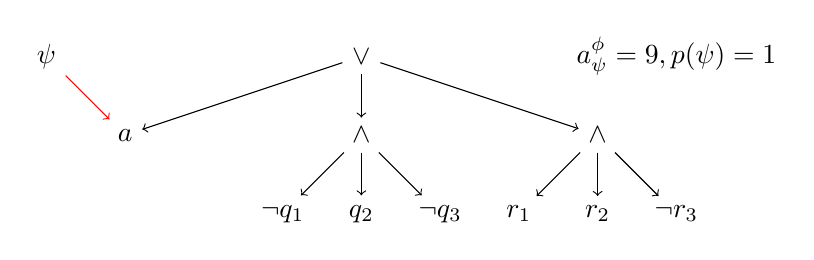
\begin{tikzpicture}
		\tikzset{vertex/.style = {}}
		\tikzset{edge/.style = {->}}
		
		\node[vertex]  (1) at (   0,    1) {$\vee$};
		\node[vertex]  (2) at (  -3,    0) {$a$};
		\node[vertex]  (3) at (   0,    0) {$\wedge$};
		\node[vertex]  (4) at (   3,    0) {$\wedge$};
		\node[vertex]  (8) at (  -1,   -1) {$\neg q_1$};
		\node[vertex]  (9) at (   0,   -1) {$q_2$};
		\node[vertex] (10) at (   1,   -1) {$\neg q_3$};
		\node[vertex] (11) at (   2,   -1) {$r_1$};
		\node[vertex] (12) at (   3,   -1) {$r_2$};
		\node[vertex] (13) at (   4,   -1) {$\neg r_3$};
		
		\node[vertex] (14) at (  -4,    1) {$\psi$};
		
		\node[vertex] (15) at (   4,    1) {$a_\psi^\phi = 9, p(\psi) = 1$};
		
		\draw[edge] (1) to  (2);
		\draw[edge] (1) to  (3);
		\draw[edge] (1) to  (4);
		\draw[edge] (3) to  (8);
		\draw[edge] (3) to  (9);
		\draw[edge] (3) to (10);
		\draw[edge] (4) to (11);
		\draw[edge] (4) to (12);
		\draw[edge] (4) to (13);
		
		\tikzset{edge/.style = {->,red}}
		\draw[edge] (14) to (2);
		\end{tikzpicture}
	\end{figure}
	
	$a \rightarrow (\neg p_1 \wedge p_2 \wedge p_3)$
\end{frame}

\begin{frame}{Reduzindo o número de cláusulas}{Algoritmo de Boy de la Tour -- Exemplo}
	\begin{figure}
		\centering
		
		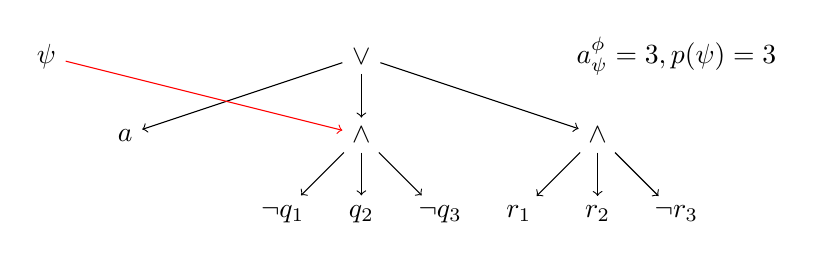
\begin{tikzpicture}
		\tikzset{vertex/.style = {}}
		\tikzset{edge/.style = {->}}
		
		\node[vertex]  (1) at (   0,    1) {$\vee$};
		\node[vertex]  (2) at (  -3,    0) {$a$};
		\node[vertex]  (3) at (   0,    0) {$\wedge$};
		\node[vertex]  (4) at (   3,    0) {$\wedge$};
		\node[vertex]  (8) at (  -1,   -1) {$\neg q_1$};
		\node[vertex]  (9) at (   0,   -1) {$q_2$};
		\node[vertex] (10) at (   1,   -1) {$\neg q_3$};
		\node[vertex] (11) at (   2,   -1) {$r_1$};
		\node[vertex] (12) at (   3,   -1) {$r_2$};
		\node[vertex] (13) at (   4,   -1) {$\neg r_3$};
		
		\node[vertex] (14) at (  -4,    1) {$\psi$};
		
		\node[vertex] (15) at (   4,    1) {$a_\psi^\phi = 3, p(\psi) = 3$};
		
		\draw[edge] (1) to  (2);
		\draw[edge] (1) to  (3);
		\draw[edge] (1) to  (4);
		\draw[edge] (3) to  (8);
		\draw[edge] (3) to  (9);
		\draw[edge] (3) to (10);
		\draw[edge] (4) to (11);
		\draw[edge] (4) to (12);
		\draw[edge] (4) to (13);
		
		\tikzset{edge/.style = {->,red}}
		\draw[edge] (14) to (3);
		\end{tikzpicture}
	\end{figure}
	
	$a \rightarrow (\neg p_1 \wedge p_2 \wedge p_3)$
\end{frame}

\begin{frame}{Reduzindo o número de cláusulas}{Algoritmo de Boy de la Tour -- Exemplo}
	\begin{figure}
		\centering
		
		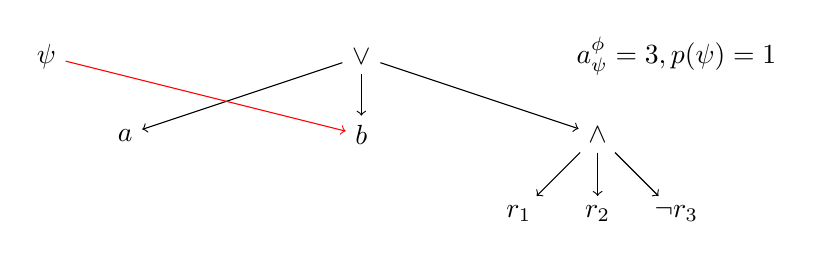
\begin{tikzpicture}
		\tikzset{vertex/.style = {}}
		\tikzset{edge/.style = {->}}
		
		\node[vertex]  (1) at (   0,    1) {$\vee$};
		\node[vertex]  (2) at (  -3,    0) {$a$};
		\node[vertex]  (3) at (   0,    0) {$b$};
		\node[vertex]  (4) at (   3,    0) {$\wedge$};
		\node[vertex] (11) at (   2,   -1) {$r_1$};
		\node[vertex] (12) at (   3,   -1) {$r_2$};
		\node[vertex] (13) at (   4,   -1) {$\neg r_3$};
		
		\node[vertex] (14) at (  -4,    1) {$\psi$};
		
		\node[vertex] (15) at (   4,    1) {$a_\psi^\phi = 3, p(\psi) = 1$};
		
		\draw[edge] (1) to  (2);
		\draw[edge] (1) to  (3);
		\draw[edge] (1) to  (4);
		\draw[edge] (4) to (11);
		\draw[edge] (4) to (12);
		\draw[edge] (4) to (13);
		
		\tikzset{edge/.style = {->,red}}
		\draw[edge] (14) to (3);
		\end{tikzpicture}
	\end{figure}
	
	$a \rightarrow (\neg p_1 \wedge p_2 \wedge p_3)$\\
	$b \rightarrow (\neg q_1 \wedge q_2 \wedge \neg q_3)$
\end{frame}

\begin{frame}{Reduzindo o número de cláusulas}{Algoritmo de Boy de la Tour -- Exemplo}
	\begin{figure}
		\centering
		
		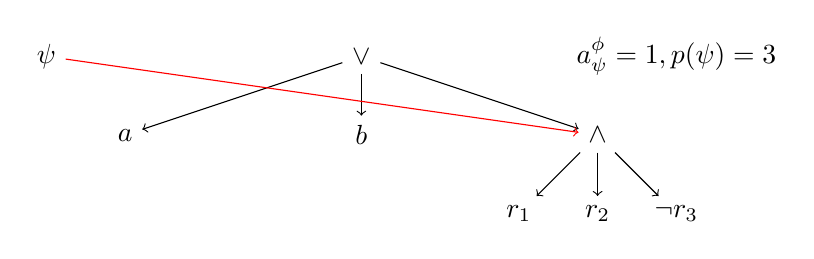
\begin{tikzpicture}
		\tikzset{vertex/.style = {}}
		\tikzset{edge/.style = {->}}
		
		\node[vertex]  (1) at (   0,    1) {$\vee$};
		\node[vertex]  (2) at (  -3,    0) {$a$};
		\node[vertex]  (3) at (   0,    0) {$b$};
		\node[vertex]  (4) at (   3,    0) {$\wedge$};
		\node[vertex] (11) at (   2,   -1) {$r_1$};
		\node[vertex] (12) at (   3,   -1) {$r_2$};
		\node[vertex] (13) at (   4,   -1) {$\neg r_3$};
		
		\node[vertex] (14) at (  -4,    1) {$\psi$};
		
		\node[vertex] (15) at (   4,    1) {$a_\psi^\phi = 1, p(\psi) = 3$};
		
		\draw[edge] (1) to  (2);
		\draw[edge] (1) to  (3);
		\draw[edge] (1) to  (4);
		\draw[edge] (4) to (11);
		\draw[edge] (4) to (12);
		\draw[edge] (4) to (13);
		
		\tikzset{edge/.style = {->,red}}
		\draw[edge] (14) to (4);
		\end{tikzpicture}
	\end{figure}
	
	$a \rightarrow (\neg p_1 \wedge p_2 \wedge p_3)$\\
	$b \rightarrow (\neg q_1 \wedge q_2 \wedge \neg q_3)$
\end{frame}

\begin{frame}{Reduzindo o número de cláusulas}{Algoritmo de Boy de la Tour -- Exemplo}
	$$(a \vee b \vee (r_1 \wedge r_2 \wedge \neg r_3)) \wedge (a \rightarrow (\neg p_1 \wedge p_2 \wedge p_3)) \wedge (b \rightarrow (\neg q_1 \wedge q_2 \wedge \neg q_3))$$
	
	\pause Número de cláusulas: 9
\end{frame}
